% Preamble templated from Mihir-Divyansh/Course-Setup
%iffalse
\let\negmedspace\undefined
\let\negthickspace\undefined
\documentclass[journal,12pt,onecolumn]{IEEEtran}
\usepackage{cite}
\usepackage{amsmath,amssymb,amsfonts,amsthm}
\usepackage{algorithmic}
\usepackage{graphicx}
\usepackage{textcomp}
\usepackage{xcolor}
\usepackage{txfonts}
\usepackage{listings}
\usepackage{enumitem}
\usepackage{mathtools}
\usepackage{gensymb}
\usepackage{comment}
\usepackage[breaklinks=true]{hyperref}
\usepackage{tkz-euclide}
\usepackage{listings}
\usepackage{gvv}
%\def\inputGnumericTable{}
\usepackage[latin1]{inputenc}
\usepackage{color}
\usepackage{array}
\usepackage{longtable}
\usepackage{calc}
\usepackage{multirow}
\usepackage{hhline}
\usepackage{ifthen}
\usepackage{lscape}
\usepackage{tabularx}
\usepackage{array}
\usepackage{float}
\usepackage{caption}
\usepackage{multicol}

\newtheorem{theorem}{Theorem}[section]
\newtheorem{problem}{Problem}
\newtheorem{proposition}{Proposition}[section]
\newtheorem{lemma}{Lemma}[section]
\newtheorem{corollary}[theorem]{Corollary}
\newtheorem{example}{Example}[section]
\newtheorem{definition}[problem]{Definition}
\newcommand{\BEQA}{\begin{eqnarray}}
\newcommand{\EEQA}{\end{eqnarray}}
\newcommand{\define}{\stackrel{\triangle}{=}}
\theoremstyle{remark}
\newtheorem{rem}{Remark}

% Marks the beginning of the document
\begin{document}
\bibliographystyle{IEEEtran}
\vspace{3cm}

\title{Assignment 3: GATE 2018 PH: Physics}
\author{EE25BTECH11055 - Subhodeep Chakraborty}
\maketitle
\hrulefill
\bigskip

\renewcommand{\thefigure}{\theenumi}
\renewcommand{\thetable}{\theenumi}


\begin{enumerate}
    \item "When she fell down the \rule{1cm}{0.4pt}, she received many \rule{1cm}{0.4pt} but little help."
    The words that best fill the blanks in the above sentence are
    \hfill\brak{\text{GATE PH 2018}} \begin{enumerate}
        \item stairs, stares
        \item stairs, stairs
        \item stares, stairs
        \item stares, stares
    \end{enumerate}

    \item "In spite of being warned repeatedly, he failed to correct his \rule{1cm}{0.4pt} behaviour."
    The word that best fills the blank in the above sentence is
    \hfill\brak{\text{GATE PH 2018}} \begin{enumerate}
        \item rational
        \item reasonable
        \item errant
        \item good
    \end{enumerate}

    \item For $0 \le x \le 2\pi$, $\sin x$ and $\cos x$ are both decreasing functions in the interval
    \hfill\brak{\text{GATE PH 2018}} \begin{enumerate}
        \item $(0, \frac{\pi}{2})$
        \item $(\frac{\pi}{2}, \pi)$
        \item $(\pi, \frac{3\pi}{2})$
        \item $(\frac{3\pi}{2}, 2\pi)$
    \end{enumerate}

    \item The area of an equilateral triangle is $\sqrt{3}$. What is the perimeter of the triangle?
    \hfill\brak{\text{GATE PH 2018}} \begin{enumerate}
        \item 2
        \item 4
        \item 6
        \item 8
    \end{enumerate}

    \item Arrange the following three-dimensional objects in the descending order of their volumes:
    \hfill\brak{\text{GATE PH 2018}} \begin{enumerate}
        \item A cuboid with dimensions 10 cm, 8 cm and 6 cm
        \item A cube of side 8 cm
        \item A cylinder with base radius 7 cm and height 7 cm
        \item A sphere of radius 7 cm
    \end{enumerate}
    \hfill\brak{\text{GATE PH 2018}} \begin{enumerate}
        \item a, b, c, d
        \item b, a, d, c
        \item c, b, a, d
        \item d, c, b, a
    \end{enumerate}

    \item An automobile travels from city A to city B and returns to city A by the same route. The speed of the vehicle during the onward and return journeys were constant at $60 \text{ km/h}$ and $90 \text{ km/h}$ respectively. What is the average speed in km/h for the entire journey?
    \hfill\brak{\text{GATE PH 2018}} \begin{enumerate}
        \item 72
        \item 73
        \item 74
        \item 75
    \end{enumerate}

    \item A set of 4 parallel lines intersect with another set of 5 parallel lines. How many parallelograms are formed?
    \hfill\brak{\text{GATE PH 2018}} \begin{enumerate}
        \item 20
        \item 48
        \item 60
        \item 72
    \end{enumerate}

    \item To pass a test, a candidate needs to answer at least 2 out of 3 questions correctly. A total of 6,30,000 candidates appeared for the test. Question A was correctly answered by 3,30,000 candidates. Question B was answered correctly by 2,50,000 candidates. Question C was answered correctly by 2,60,000 candidates. Both questions A and B were answered correctly by 1,00,000 candidates. Both questions B and C were answered correctly by 90,000 candidates. Both questions A and C were answered correctly by 80,000 candidates. If the number of students answering all questions correctly is the same as the number answering none, how many candidates failed to clear the test?
    \hfill\brak{\text{GATE PH 2018}} \begin{enumerate}
        \item 30,000
        \item 2,70,000
        \item 3,90,000
        \item 4,20,000
    \end{enumerate}

    \item If $x^2 + x - 1 = 0$ what is the value of $x^4 + \frac{1}{x^4}$?
    \hfill\brak{\text{GATE PH 2018}} \begin{enumerate}
        \item 1
        \item 5
        \item 7
        \item 9
    \end{enumerate}

    \item In a detailed study of annual crow births in India, it was found that there was relatively no growth during the period 2002 to 2004 and a sudden spike from 2004 to 2005. In another unrelated study, it was found that the revenue from cracker sales in India which remained fairly flat from 2002 to 2004, saw a sudden spike in 2005 before declining again in 2006. The solid line in the graph below in \figref{fig:10} refers to annual sale of crackers and the dashed line refers to the annual crow births in India. Choose the most appropriate inference from the above data.

    \begin{figure}[H]
        \centering
        \caption{} \label{fig:10} 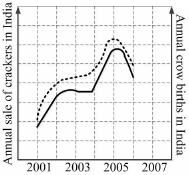
\includegraphics{figs/10.png}
    \end{figure}

    \hfill\brak{\text{GATE PH 2018}} \begin{enumerate}
        \item There is a strong correlation between crow birth and cracker sales.
        \item Cracker usage increases crow birth rate.
        \item If cracker sale declines, crow birth will decline.
        \item Increased birth rate of crows will cause an increase in the sale of crackers.
    \end{enumerate}

\newpage

    \item The eigenvalues of a Hermitian matrix are all
 \hfill\brak{\text{GATE PH 2018}} \begin{enumerate}
        \item real
        \item imaginary
        \item of modulus one
        \item real and positive
    \end{enumerate}

    \item Which one of the following represents the 3p radial wave function of hydrogen atom? ($a_0$ is the Bohr radius)\hfill\brak{\text{GATE PH 2018}}

    \begin{figure}[H]
        \centering
        \caption*{} \label{fig:12o} 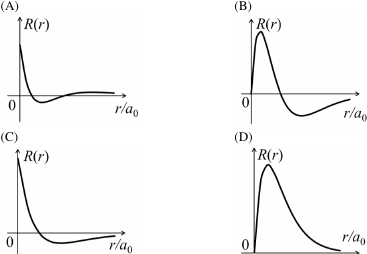
\includegraphics{figs/12.png}
    \end{figure}

    \item Given the following table, which one of the following correctly matches the experiments from Group I to their inferences in Group II?
    \begin{center}
    \begin{tabular}{|l|l|}
        \hline
        \textbf{Group I} & \textbf{Group II} \\
        \hline
        P: Stern-Gerlach experiment & 1: Wave nature of particles \\
        \hline
        Q: Zeeman effect & 2: Quantization of energy of electrons in the atoms \\
        \hline
        R: Frank-Hertz experiment & 3: Existence of electron spin \\
        \hline
        S: Davisson-Germer experiment & 4: Space quantization of angular momentum \\
        \hline
    \end{tabular}
    \end{center}
    \hfill\brak{\text{GATE PH 2018}} \begin{enumerate}
        \item P-2, Q-3, R-4, S-1
        \item P-1, Q-3, R-2, S-4
        \item P-3, Q-4, R-2, S-1
        \item P-2, Q-1, R-4, S-3
    \end{enumerate}

    \item In spherical polar coordinates $(r, \theta, \phi)$, the unit vector $\hat{\theta}$ at \brak{10, \pi/4, \pi/2} is
    \hfill\brak{\text{GATE PH 2018}} \begin{enumerate}
        \item $\hat{k}$
        \item $\frac{1}{\sqrt{2}}(\hat{j}+\hat{k})$
        \item $\frac{1}{\sqrt{2}}(-\hat{j}+\hat{k})$
        \item $\frac{1}{\sqrt{2}}(\hat{j}-\hat{k})$
    \end{enumerate}

    \item The scale factors corresponding to the covariant metric tensor $g_{ij}$ in spherical polar coordinates are
    \hfill\brak{\text{GATE PH 2018}} \begin{enumerate}
        \item $1, r^2, r^2 \sin^2\theta$
        \item $1, r^2, \sin^2\theta$
        \item $1, 1, 1$
        \item $1, r, r \sin\theta$
    \end{enumerate}

    \item In the context of small oscillations, which one of the following does NOT apply to the normal coordinates?
    \hfill\brak{\text{GATE PH 2018}} \begin{enumerate}
        \item Each normal coordinate has an eigen-frequency associated with it
        \item The normal coordinates are orthogonal to one another
        \item The normal coordinates are all independent
        \item The potential energy of the system is a sum of squares of the normal coordinates with constant coefficients
    \end{enumerate}

    \item For the given unit cells of a two dimensional square lattice in \figref{fig:17} which option lists all the primitive cells?

    \begin{figure}[H]
        \centering
        \caption{} \label{fig:17} 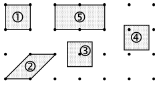
\includegraphics{figs/17.png}
    \end{figure} \hfill\brak{\text{GATE PH 2018}}
\begin{enumerate}
 \item 1 and 2
 \item 1, 2 and 3
 \item 1, 2, 3 and 4
 \item 1, 2, 3, 4 and 5
\end{enumerate}

    \item Among electric field $(\vec{E})$, magnetic field $(\vec{B})$, angular momentum $(\vec{L})$, and vector potential $(\vec{A})$, which is/are odd under parity (space inversion) operation?
    \hfill\brak{\text{GATE PH 2018}} \begin{enumerate}
        \item $\vec{E}$ only
        \item $\vec{E}$ \& $\vec{A}$ only
        \item $\vec{E}$ \& $\vec{B}$ only
        \item $\vec{B}$ \& $\vec{L}$ only
    \end{enumerate}

    \item The expression for the second overtone frequency in the vibrational absorption spectra of a diatomic molecule in terms of the harmonic frequency $\omega_e$ and anharmonicity constant $x_e$ is
    \hfill\brak{\text{GATE PH 2018}} \begin{enumerate}
        \item $2\omega_e(1-x_e)$
        \item $2\omega_e(1-3x_e)$
        \item $3\omega_e(1-2x_e)$
        \item $3\omega_e(1-4x_e)$
    \end{enumerate}

    \item Match the physical effects and order of magnitude of their energy scales given below, where $\alpha = \frac{e^2}{4\pi\epsilon_0\hbar c}$ is fine structure constant; $m_e$ and $m_p$ are electron and proton mass, respectively.
    \begin{center}
    \begin{tabular}{|l|l|}
        \hline
        \textbf{Group I} & \textbf{Group II} \\
        \hline
        P: Lamb shift & 1: $\sim O(\alpha^2 m_e c^2)$ \\ \hline
        Q: Fine structure & 2: $\sim O(\alpha^4 m_e c^2)$ \\ \hline
        R: Bohr energy & 3: $\sim O(\alpha^4 m_e^2 c^2/m_p)$ \\ \hline
        S: Hyperfine structure & 4: $\sim O(\alpha^5 m_e c^2)$ \\
        \hline
    \end{tabular}
    \end{center}
    \hfill\brak{\text{GATE PH 2018}} \begin{enumerate}
        \item P-3, Q-1, R-2, S-4
        \item P-2, Q-3, R-1, S-4
        \item P-4, Q-2, R-1, S-3
        \item P-2, Q-4, R-1, S-3
    \end{enumerate}

    \item The logic expression $\overline{A}BC + \overline{A}\overline{B}C + AB\overline{C} + A\overline{B}\overline{C}$ can be simplified to
    \hfill\brak{\text{GATE PH 2018}} \begin{enumerate}
        \item A XOR C
        \item A AND C
        \item 0
        \item 1
    \end{enumerate}

    \item At low temperatures (T), the specific heat of common metals is described by (with $\alpha$ and $\beta$ as constants)
    \hfill\brak{\text{GATE PH 2018}} \begin{enumerate}
        \item $\alpha T + \beta T^3$
        \item $\beta T^3$
        \item $\exp(-\alpha/T)$
        \item $\alpha T + \beta T^5$
    \end{enumerate}

    \item In a 2-to-1 multiplexer as shown below in \figref{fig:23}, the output $X = A_0$ if $C=0$, and $X = A_1$ if $C=1$.
    \begin{figure}[H]
        \centering
        \caption{} \label{fig:23} 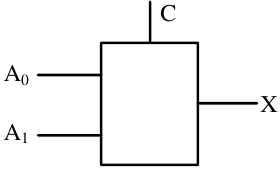
\includegraphics{figs/23.png}
    \end{figure}
    Which one of the following is the correct implementation of this multiplexer? \hfill\brak{\text{GATE PH 2018}}
    \begin{figure}[H]
        \centering
\caption*{} \label{fig:23o} 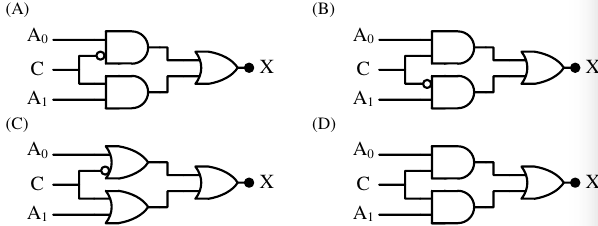
\includegraphics{figs/23o.png}
\end{figure}

    \item The elementary particle $\Xi^0$ is placed in the baryon decuplet, shown below in \figref{fig:24}, at
    \begin{figure}[H]
        \centering
        \caption{} \label{fig:24} 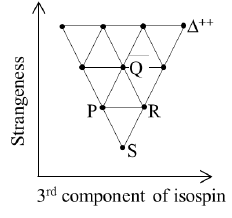
\includegraphics{figs/24.png}
    \end{figure}
    \hfill\brak{\text{GATE PH 2018}} \begin{enumerate}
        \item P
        \item Q
        \item R
        \item S
    \end{enumerate}

    \item The intrinsic/permanent electric dipole moment in the ground state of hydrogen atom is ($a_0$ is the Bohr radius)
    \hfill\brak{\text{GATE PH 2018}} \begin{enumerate}
        \item $-3ea_0$
        \item zero
        \item $ea_0$
        \item $3ea_0$
    \end{enumerate}

    \item The high temperature magnetic susceptibility of solids having ions with magnetic moments can be described by $\chi \propto \frac{1}{T+\theta}$ with T as absolute temperature and $\theta$ as constant. The three behaviors i.e. paramagnetic, ferromagnetic and anti-ferromagnetic are described, respectively, by
    \hfill\brak{\text{GATE PH 2018}} \begin{enumerate}
        \item $\theta<0, \theta>0, \theta=0$
        \item $\theta>0, \theta<0, \theta=0$
        \item $\theta=0, \theta<0, \theta>0$
        \item $\theta=0, \theta>0, \theta<0$
    \end{enumerate}

    \item Which one of the following is an allowed electric dipole transition?
    \hfill\brak{\text{GATE PH 2018}} \begin{enumerate}
        \item ${}^3S_1 \rightarrow {}^3S_1$
        \item ${}^2P_{3/2} \rightarrow {}^2D_{5/2}$
        \item ${}^2D_{5/2} \rightarrow {}^2P_{1/2}$
        \item ${}^3P_0 \rightarrow {}^5D_0$
    \end{enumerate}

    \item In the decay, $\mu^+ \rightarrow e^+ + \nu_e + X$, what is X?
    \hfill\brak{\text{GATE PH 2018}} \begin{enumerate}
        \item $\gamma$
        \item $\overline{\nu}_e$
        \item $\nu_\mu$
        \item $\overline{\nu}_\mu$
    \end{enumerate}

    \item A spaceship is travelling with a velocity of 0.7c away from a space station. The spaceship ejects a probe with a velocity 0.59c opposite to its own velocity. A person in the space station would see the probe moving at a speed Xc, where the value of X is \rule{1cm}{0.4pt} (up to three decimal places).
\hfill\brak{\text{GATE PH 2018}}
    \item For an operational amplifier (ideal) circuit shown below in \figref{fig:30}, if $V_1 = 1$ V and $V_2 = 2$ V, the value of $V_0$ is \rule{1cm}{0.4pt} V (up to one decimal place).
    \begin{figure}[H]
        \centering
        \caption{} \label{fig:30} 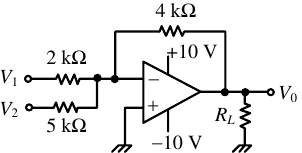
\includegraphics{figs/30.png}
    \end{figure}\hfill\brak{\text{GATE PH 2018}}

    \item An infinitely long straight wire is carrying a steady current I. The ratio of magnetic energy density at distance $r_1$ to that at $r_2 (= 2r_1)$ from the wire is \rule{1cm}{0.4pt}.\hfill\brak{\text{GATE PH 2018}}

    \item A light beam of intensity $I_0$ is falling normally on a surface. The surface absorbs 20\% of the intensity and the rest is reflected. The radiation pressure on the surface is given by $X I_0/c$, where X is \rule{1cm}{0.4pt} (up to one decimal place). Here c is the speed of light.\hfill\brak{\text{GATE PH 2018}}

    \item The number of independent components of a general electromagnetic field tensor is \rule{1cm}{0.4pt}. \hfill\brak{\text{GATE PH 2018}}

    \item If X is the dimensionality of a free electron gas, the energy (E) dependence of density of states is given by $E^{\frac{1}{2}X-Y}$, where Y is \rule{1cm}{0.4pt}.\hfill\brak{\text{GATE PH 2018}}

    \item For nucleus $^{164}\text{Er}$ a $J^\pi=2^+$ state is at 90 keV. Assuming $^{164}\text{Er}$ to be a rigid rotor, the energy of its $4^+$ state is \rule{1cm}{0.4pt} keV (up to one decimal place).\hfill\brak{\text{GATE PH 2018}}

    \item Given $\vec{V}_1 = \hat{i} - \hat{j}$ and $\vec{V}_2 = -2\hat{i} + 3\hat{j} + 2\hat{k}$, which one of the following $\vec{V}_3$ makes $(\vec{V}_1, \vec{V}_2, \vec{V}_3)$ a complete set for a three dimensional real linear vector space?
    \hfill\brak{\text{GATE PH 2018}} \begin{enumerate}
        \item $\vec{V}_3 = \hat{i} + \hat{j} + 4\hat{k}$
        \item $\vec{V}_3 = 2\hat{i} - \hat{j} + 2\hat{k}$
        \item $\vec{V}_3 = \hat{i} + 2\hat{j} + 6\hat{k}$
        \item $\vec{V}_3 = 2\hat{i} + \hat{j} + 4\hat{k}$
    \end{enumerate}

    \item An interstellar object has speed v at the point of its shortest distance R from a star of much larger mass M. Given $v^2 = 2GM/R$, the trajectory of the object is
    \hfill\brak{\text{GATE PH 2018}} \begin{enumerate}
        \item circle
        \item ellipse
        \item parabola
        \item hyperbola
    \end{enumerate}

    \item A particle moves in one dimension under a potential $V(x) = \alpha |x|$ with some non-zero total energy. Which one of the following best describes the particle trajectory in the phase space?\hfill\brak{\text{GATE PH 2018}}
    \begin{figure}[H]
        \centering
        \caption*{} \label{fig:38o} 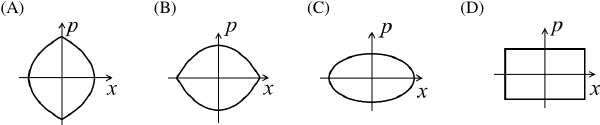
\includegraphics{figs/38.png}
    \end{figure}

    \item Consider an infinitely long solenoid with N turns per unit length, radius R and carrying a current $I(t) = \alpha \cos \omega t$, where $\alpha$ is a constant and $\omega$ is the angular frequency. The magnitude of electric field at the surface of the solenoid is
    \hfill\brak{\text{GATE PH 2018}} \begin{enumerate}
        \item $\frac{1}{2} \mu_0 N R \omega \alpha \sin \omega t$
        \item $\frac{1}{2} \mu_0 \omega N R \cos \omega t$
        \item $\mu_0 N R \omega \alpha \sin \omega t$
        \item $\mu_0 \omega N R \cos \omega t$
    \end{enumerate}

    \item A constant and uniform magnetic field $\vec{B} = B_0 \hat{k}$ pervades all space. Which one of the following is the correct choice for the vector potential in Coulomb gauge?
    \hfill\brak{\text{GATE PH 2018}} \begin{enumerate}
        \item $-B_0(x+y)\hat{i}$
        \item $B_0(x+y)\hat{j}$
        \item $B_0 x \hat{j}$
        \item $-\frac{1}{2}B_0(x\hat{i} - y\hat{j})$
    \end{enumerate}

    \item If H is the Hamiltonian for a free particle with mass m, the commutator $[x, [x, H]]$ is
    \hfill\brak{\text{GATE PH 2018}} \begin{enumerate}
        \item $\hbar^2/m$
        \item $-\hbar^2/m$
        \item $-\hbar^2/(2m)$
        \item $\hbar^2/(2m)$
    \end{enumerate}

    \item A long straight wire, having radius a and resistance per unit length r, carries a current I. The magnitude and direction of the Poynting vector on the surface of the wire is
    \hfill\brak{\text{GATE PH 2018}} \begin{enumerate}
        \item $I^2r/(2\pi a)$, perpendicular to axis of the wire and pointing inwards
        \item $I^2r/(2\pi a)$, perpendicular to axis of the wire and pointing outwards
        \item $I^2r/(\pi a)$, perpendicular to axis of the wire and pointing inwards
        \item $I^2r/(\pi a)$, perpendicular to axis of the wire and pointing outwards
    \end{enumerate}

    \item Three particles are to be distributed in four non-degenerate energy levels. The possible number of ways of distribution: (i) for distinguishable particles, and (ii) for identical Bosons, respectively, is
    \hfill\brak{\text{GATE PH 2018}} \begin{enumerate}
        \item (i) 24, (ii) 4
        \item (i) 24, (ii) 20
        \item (i) 64, (ii) 20
        \item (i) 64, (ii) 16
    \end{enumerate}

    \item The term symbol for the electronic ground state of oxygen atom is
    \hfill\brak{\text{GATE PH 2018}} \begin{enumerate}
        \item $^1S_0$
        \item $^1D_2$
        \item $^3P_0$
        \item $^3P_2$
    \end{enumerate}

    \item The energy dispersion for electrons in one dimensional lattice with lattice parameter a is given by $E(k) = E_0 - \frac{1}{2}W \cos ka$, where W and $E_0$ are constants. The effective mass of the electron near the bottom of the band is
    \hfill\brak{\text{GATE PH 2018}} \begin{enumerate}
        \item $\frac{2\hbar^2}{Wa^2}$
        \item $\frac{\hbar^2}{Wa^2}$
        \item $\frac{\hbar^2}{2Wa^2}$
        \item $\frac{\hbar^2}{4Wa^2}$
    \end{enumerate}

    \item Amongst electrical resistivity ($\rho$), thermal conductivity ($\kappa$), specific heat (C), Young's modulus (Y), and magnetic susceptibility ($\chi$), which quantities show a sharp change at the superconducting transition temperature?
    \hfill\brak{\text{GATE PH 2018}} \begin{enumerate}
        \item $\rho, \kappa, C, \chi$
        \item $\rho, C, \chi$
        \item $\rho, \kappa, Y, \chi$
        \item $\kappa, Y, \chi$
    \end{enumerate}

    \item A quarter wave plate introduces a path difference of $\lambda/4$ between the two components of polarization parallel and perpendicular to the optic axis. An electromagnetic wave with $\vec{E} = (\hat{x} + \hat{y})E_0 e^{i(kz-\omega t)}$ is incident normally on a quarter wave plate which has its optic axis making an angle $135\degree$ with the x-axis as shown in \figref{fig:47}. The emergent electromagnetic wave would be
    \begin{figure}[H]
        \centering
        \caption{} \label{fig:47} 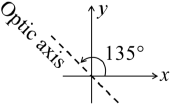
\includegraphics{figs/47.png}
    \end{figure}
    \hfill\brak{\text{GATE PH 2018}} \begin{enumerate}
        \item elliptically polarized
        \item circularly polarized
        \item linearly polarized with polarization as that of incident wave
        \item linearly polarized but with polarization at $90\degree$ to that of the incident wave
    \end{enumerate}

    \item A p-doped semiconductor slab carries a current $I = 100$ mA in a magnetic field $B=0.2$ T as shown in \figref{fig:48}. One measures $V_y = 0.25$ mV and $V_x = 2$ mV. The mobility of holes in the semiconductor is \rule{1.5cm}{0.4pt} m$^2$V$^{-1}$s$^{-1}$ (up to two decimal places).
    \begin{figure}[H]
        \centering
        \caption{} \label{fig:48} 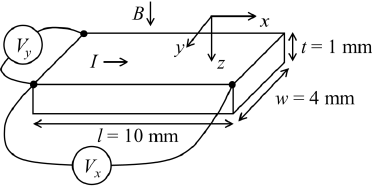
\includegraphics{figs/48.png}
    \end{figure}\hfill\brak{\text{GATE PH 2018}}

    \item An n-channel FET having Gate-Source switch-off voltage $V_{GS(OFF)} = -2$ V is used to invert a 0-5 V square-wave signal as shown in \figref{fig:49}. The maximum allowed value of R would be \rule{1.5cm}{0.4pt} k$\Omega$ (up to two decimal places).
    \begin{figure}[H]
        \centering
        \caption{} \label{fig:49} 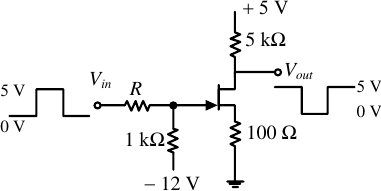
\includegraphics{figs/49.png}
    \end{figure}\hfill\brak{\text{GATE PH 2018}}

    \item Inside a large nucleus, a nucleon with mass 939 MeVc$^{-2}$ has Fermi momentum 1.40 fm$^{-1}$ at absolute zero temperature. Its velocity is Xc, where the value of X is \rule{1.5cm}{0.4pt} (up to two decimal places). ($\hbar c = 197$ MeV-fm)\hfill\brak{\text{GATE PH 2018}}

    \item 4 MeV $\gamma$-rays emitted by the de-excitation of $^{19}$F are attributed, assuming spherical symmetry, to the transition of protons from $1d_{3/2}$ state to $1d_{5/2}$ state. If the contribution of spin-orbit term to the total energy is written as $C\langle\vec{l} \cdot \vec{s}\rangle$, the magnitude of C is \rule{1.5cm}{0.4pt} MeV (up to one decimal place).\hfill\brak{\text{GATE PH 2018}}

    \item An $\alpha$ particle is emitted by a ${}^{230}_{90}\text{Th}$ nucleus. Assuming the potential to be purely Coulombic beyond the point of separation, the height of the Coulomb barrier is \rule{1.5cm}{0.4pt} MeV (up to two decimal places). ($e^2/(4\pi\epsilon_0) = 1.44$ MeV-fm, $r_0 = 1.30$ fm)\hfill\brak{\text{GATE PH 2018}}

    \item For the transformation \begin{align*} Q = \sqrt{2q} e^{-1+2\alpha\cos p}, P = \sqrt{2q} e^{-\alpha-1}\sin p\end{align*} (where $\alpha$ is a constant) to be canonical, the value of $\alpha$ is \rule{1.5cm}{0.4pt}.\hfill\brak{\text{GATE PH 2018}}

    \item Given \begin{align*}\frac{d^2f(x)}{dx^2} - 2\frac{df(x)}{dx} + f(x) = 0\end{align*}, and boundary conditions $f(0)=1$ and $f(1)=0$, the value of $f(0.5)$ is \rule{1.5cm}{0.4pt} (up to two decimal places).\hfill\brak{\text{GATE PH 2018}}

    \item The absolute value of the integral \begin{align*}\oint \frac{5z^3 + 3z^2}{z^2-4} dz\end{align*}, over the circle $|z-1.5|=1$ in complex plane, is \rule{1.5cm}{0.4pt} (up to two decimal places).\hfill\brak{\text{GATE PH 2018}}

    \item A uniform circular disc of mass $m$ and radius $R$ is rotating with angular speed $\omega$ about an axis passing through its center and making an angle $\theta=30\degree$ with the axis of the disc. If the kinetic energy of the disc is $\alpha m \omega^2 R^2$, the value of $\alpha$ is \rule{1.5cm}{0.4pt} (up to 2 decimal places).
    \begin{figure}[H]
        \centering
        \caption*{} \label{fig:56} 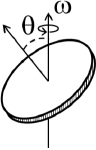
\includegraphics{figs/56.png}
    \end{figure}\hfill\brak{\text{GATE PH 2018}}

    \item The ground state energy of a particle of mass $m$ in an infinite potential well is $E_0$. It changes to $E_0(1 + \alpha \times 10^{-3})$, when there is a small potential bump of height $V_0 = \frac{\pi^2\hbar^2}{50mL^2}$ and width $a = L/100$, as shown in \figref{fig:57}. The value of $\alpha$ is \rule{1.5cm}{0.4pt} (up to two decimal places).
    \begin{figure}[H]
        \centering
        \caption{} \label{fig:57} 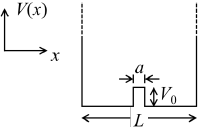
\includegraphics{figs/57.png}
    \end{figure}\hfill\brak{\text{GATE PH 2018}}

    \item An electromagnetic plane wave is propagating with an intensity $I = 1.0 \times 10^5 \text{ Wm}^{-2}$ in a medium with $\epsilon = 3\epsilon_0$ and $\mu = \mu_0$. The amplitude of the electric field inside the medium is \rule{1.5cm}{0.4pt} $\times 10^3 \text{ Vm}^{-1}$ (up to one decimal place). ($\epsilon_0 = 8.85 \times 10^{-12} \text{ C}^2\text{N}^{-1}\text{m}^{-2}, \mu_0 = 4\pi \times 10^{-7} \text{NA}^{-2}, c = 3 \times 10^8 \text{ ms}^{-1}$)\hfill\brak{\text{GATE PH 2018}}

    \item A microcanonical ensemble consists of 12 atoms with each taking either energy 0 state, or energy $\epsilon$ state. Both states are non-degenerate. If the total energy of this ensemble is $4\epsilon$, its entropy will be \rule{1.5cm}{0.4pt} $k_B$ (up to one decimal place), where $k_B$ is the Boltzmann constant.\hfill\brak{\text{GATE PH 2018}}

    \item A two-state quantum system has energy eigenvalues $\pm\epsilon$ corresponding to the normalized states $|\psi_{\pm}\rangle$. At time $t=0$, the system is in quantum state $\frac{1}{\sqrt{2}}[|\psi_+\rangle + |\psi_-\rangle]$. The probability that the system will be in the same state at $t = h/(6\epsilon)$ is \rule{1.5cm}{0.4pt} (up to two decimal places).\hfill\brak{\text{GATE PH 2018}}

    \item An air-conditioner maintains the room temperature at 27$\degree$C while the outside temperature is 47$\degree$C. The heat conducted through the walls of the room from outside to inside due to temperature difference is 7000 W. The minimum work done by the compressor of the air conditioner per unit time is \rule{1.5cm}{0.4pt} W.\hfill\brak{\text{GATE PH 2018}}

    \item Two solid spheres A and B have same emissivity. The radius of A is four times the radius of B, and temperature of A is twice the temperature of B. The ratio of the rate of heat radiated from A to that from B is \rule{1.5cm}{0.4pt}.\hfill\brak{\text{GATE PH 2018}}

    \item The partition function of an ensemble at a temperature T is \begin{align*}Z = \brak{2 \cosh \frac{\epsilon}{k_B T}}^N\end{align*}, where $k_B$ is the Boltzmann constant. The heat capacity of this ensemble at $T = \epsilon/k_B$ is $XNK_B$, where the value of X is \rule{1.5cm}{0.4pt} (up to two decimal places).\hfill\brak{\text{GATE PH 2018}}

    \item An atom in its singlet state is subjected to a magnetic field. The Zeeman splitting of its 650 nm spectral line is 0.03 nm. The magnitude of the field is \rule{1.5cm}{0.4pt} Tesla (up to two decimal places). ($e = 1.60 \times 10^{-19}$ C, $m_e = 9.11 \times 10^{-31}$ kg, $c = 3.0 \times 10^8$ ms$^{-1}$)\hfill\brak{\text{GATE PH 2018}}

    \item The quantum effects in an ideal gas become important below a certain temperature $T_Q$ when de Broglie wavelength corresponding to the root mean square thermal speed becomes equal to the inter-atomic separation. For such a gas of atoms of mass $2 \times 10^{-26}$ kg and number density $6.4 \times 10^{25} \text{ m}^{-3}$, $T_Q = \rule{1.5cm}{0.4pt} \times 10^{-3}$ K (up to one decimal place). ($k_B = 1.38 \times 10^{-23}$ J/K, $h = 6.6 \times 10^{-34}$ J-s)\hfill\brak{\text{GATE PH 2018}}
\end{enumerate}


\end{document}
